\begin{frame}{PHP in Combinatorics}
    In a party of 6 people, if you take any two members they are either friends or strangers. Then show that you can always find a group of 3 people, in which all pairs are either friends or all pairs are strangers.
\end{frame}

\begin{frame}{Solution}
    \begin{itemize}[<+->]
        \item Let us treat these 6 people as 6 points and color the line segment joining them {\color{blue}{blue}} if they are friends and {\color{red}{red}} if they are strangers.

        \item To prove the statement we need to show there exists a triangle whose all edges are of the same color.
        \item Now take any point there will be 5 line segments from it to remaining 5 points.
        \begin{figure}
            \centering
            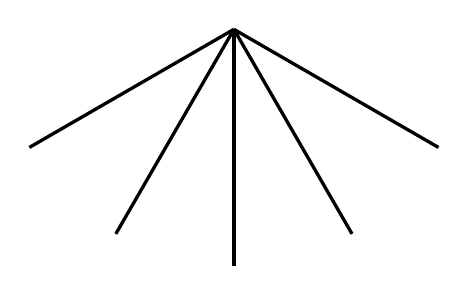
\begin{tikzpicture}
                \draw (0, 0)--(270:3) [very thick];
                \draw (0, 0)--(300:3) [very thick];
                \draw (0, 0)--(330:3) [very thick];
                \draw (0, 0)--(240:3) [very thick];
                \draw (0, 0)--(210:3) [very thick];
            \end{tikzpicture}
        \end{figure}
    \end{itemize}
\end{frame}

\begin{frame}{Solution}
    \begin{itemize}[<+->]
        \item Since we have 5 lines and 2 colors, by stronger version of PHP at least {\bf{3 of these 5}} should be of the same color say {\color{blue}{blue}}.
        \begin{figure}
            \centering
            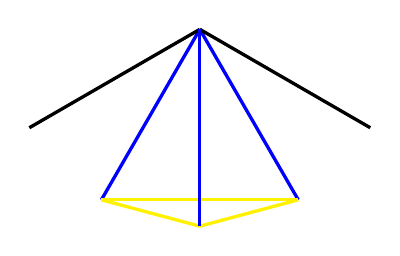
\begin{tikzpicture}
                \draw (0, 0)--(300:2.5) [blue, very thick];
                \draw (0, 0)--(330:2.5) [very thick];
                \draw (0, 0)--(240:2.5) [blue, very thick];
                \draw (0, 0)--(210:2.5) [very thick];
                \draw (270:2.5)--(300:2.5) [yellow, very thick];
                \draw (270:2.5)--(240:2.5) [yellow, very thick];
                \draw (240:2.5)--(300:2.5) [yellow, very thick];
                \draw (0, 0)--(270:2.5) [blue, very thick];
            \end{tikzpicture}
        \end{figure}
        \item If any of the {\color{yellow}{yellow}} segments are {\color{blue}{blue}} we are done.
        \item Else all of them are {\color{red}{red}}. Then we will have a {\color{red}{red}} triangle.
        \begin{figure}
            \centering
            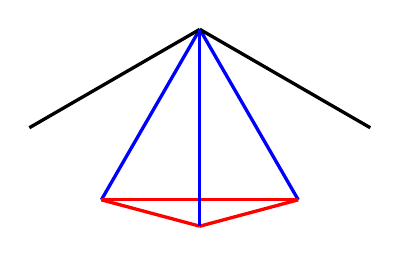
\begin{tikzpicture}
                \draw (0, 0)--(300:2.5) [blue, very thick];
                \draw (0, 0)--(330:2.5) [very thick];
                \draw (0, 0)--(240:2.5) [blue, very thick];
                \draw (0, 0)--(210:2.5) [very thick];
                \draw (270:2.5)--(300:2.5) [red, very thick];
                \draw (270:2.5)--(240:2.5) [red, very thick];
                \draw (240:2.5)--(300:2.5) [red, very thick];
                \draw (0, 0)--(270:2.5) [blue, very thick];
            \end{tikzpicture}
        \end{figure}
        \item Hence Proved!!
    \end{itemize}
\end{frame}